\documentclass[11pt]{article}

\usepackage[margin=1in]{geometry}
\usepackage[T1]{fontenc}
\usepackage[utf8]{inputenc}
\usepackage{graphicx}
\usepackage[hidelinks]{hyperref}
\usepackage{enumitem}
\usepackage{booktabs}
\usepackage{tabularx}

\graphicspath{{../data/presentation_assets/}}
\setlist{noitemsep,topsep=1pt,leftmargin=1.15em}
\setlength{\parindent}{0pt}
\setlength{\parskip}{0.10em}

\title{\vspace{-2.3em}\textbf{What Really Makes a Pokemon Strong?}\\
\large ECS 163 Progress Report}
\author{Team 13\\Team members: Yuhui Chen, Yuxiang Huang, Junhao Zhang, Jiayi Bai, Tingwei Zhang}
\date{}

\begin{document}
\maketitle
\vspace{-2.0em}

\section{Motivation, Objectives, and Current Status}

Most people first judge Pokemon by raw base stats. Our project tests that assumption in a competitive setting. We are not arguing that stats are meaningless. Instead, our claim is that raw stats matter, but competitive value also emerges from teammates, usage patterns, moves, items, abilities, support roles, and repeated team fit.

The objective is a narrative visualization that helps novice viewers understand why competitive strength is relational rather than purely statistical. The final experience follows a Martini Glass structure \cite{segel2010narrative}: it begins with a guided argument, reveals a contradiction in the data, then opens into interactive exploration. The force-directed team synergy network is the main visualization because our story is fundamentally about relationships. Supporting charts are included only when they guide the viewer toward the network explanation.

Our current implementation is more than halfway complete. We have a working React and D3 prototype with processed CSV data, a stats-vs-usage scatterplot, linked selection, scatterplot brushing, a force-directed network, hover tooltips, click selection, teammate highlighting, a reset interaction, a Pokemon picker, and a detail panel with stats, usage, rank, teammates, moves, item, and ability. The main remaining work is not adding many more charts; it is improving pacing, hierarchy, annotations, transitions, responsive polish, and the final written explanation.

\section{Driving Application and Data}

The driving application is competitive Pokemon team analysis for VGC 2022. The user-facing question is: \textit{What really makes a Pokemon strong?} This framing keeps the project from becoming a generic Pokedex browser. The visual system should help viewers compare isolated attributes, then understand why those attributes are incomplete without team context.

We use the Complete Competitive Pokemon Database (May 2022), which includes Pokemon/form records, base stats, VGC rules, monthly usage, teammate co-usage, moves, items, and abilities \cite{carbone2022competitive}. We also use a Pokemon image dataset for visual identity \cite{singh32000pokemon}. After preprocessing, the working data contains:

\begin{itemize}
  \item 1,098 Pokemon/form rows, including 228 rows with numeric usage data.
  \item 2,606 cleaned teammate co-usage edges.
  \item 2,967 build usage rows covering moves, items, and abilities.
  \item Image references for all 1,098 Pokemon/form rows.
\end{itemize}

The preprocessing step converts numeric fields, flags missing base stats, derives offensive and defensive scores, normalizes names for image lookup, keeps VGC 2022 eligibility information, filters team edges to meaningful co-usage values, and limits build rows to the most common moves, items, and abilities. This creates a coordinated-view structure: Pokemon are nodes, teammate pairs are edges, and build usage rows provide evidence for role and team function.

\begin{center}
  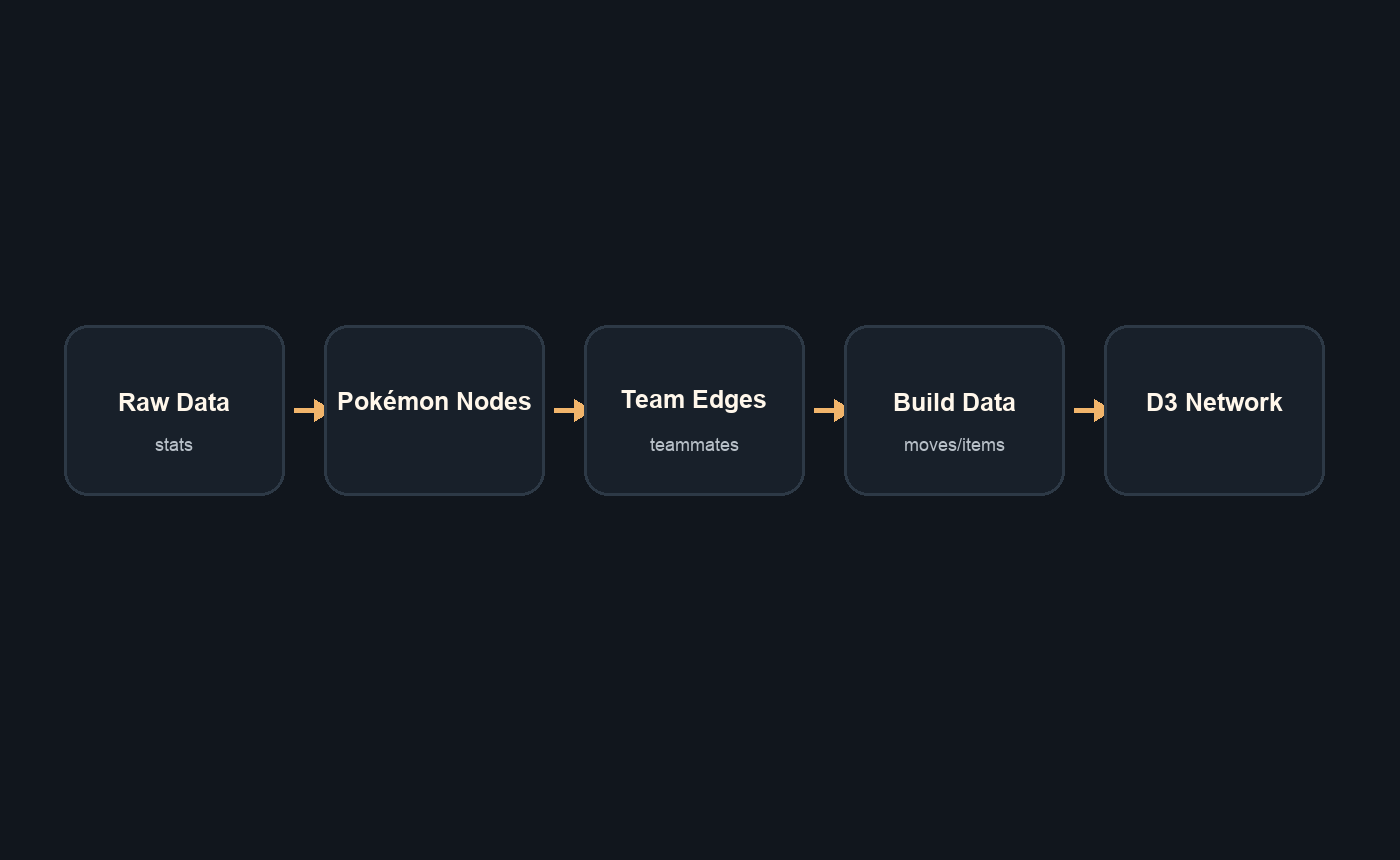
\includegraphics[width=0.70\linewidth]{dataset_pipeline.png}

  \small Figure 1. The data pipeline separates raw records into Pokemon nodes, team edges, build details, and image references so the final D3 system can coordinate views without becoming one oversized table.
\end{center}
\vspace{-0.6em}

\section{Challenges to Address and Related Work}

The main design challenge is restraint. Because the data includes stats, usage, teammates, moves, items, abilities, images, and rules, it would be easy to build a broad analytics dashboard. That would weaken the project. Our story needs controlled attention: the viewer should first see that raw stats are insufficient, then use the network to understand relational value.

We use narrative visualization principles from Segel and Heer \cite{segel2010narrative}. The guided opening provides author-driven context, while the later network interaction allows reader-driven exploration. D3 supports this structure because it gives us direct control over scales, brushing, SVG marks, force simulation, highlighting, and transitions \cite{d3js}. React manages application state and keeps the scatterplot, network, picker, and detail panel synchronized \cite{react}.

The biggest remaining risks are readability and pacing. Force-directed networks can become visually dense, so we are limiting the network to a meaningful competitive subset, using selection-based fading, adding labels only when they clarify the story, and treating the detail panel as an explanation surface rather than a separate dashboard. Another risk is overclaiming: usage is a proxy for competitive relevance, not a perfect measure of strength. The final report and interface will state this limitation clearly.

\section{Method: Design and Implementation}

Our current design has four story beats. First, the introduction states the common assumption: stronger Pokemon simply have higher stats. Second, the stats-vs-usage scatterplot shows the contradiction. Zacian Crowned Sword has high stats and high usage, but Zamazenta Crowned Shield and Mewtwo show that high stats can still produce low usage; Incineroar has moderate stats but high usage and connectivity. Third, the force-directed network reveals why: competitive value appears through repeated teammate links, support roles, and team fit. Fourth, the user can explore by clicking Pokemon, brushing regions in the scatterplot, and reading the detail panel.

The force-directed network remains the main character. Nodes represent Pokemon, node size encodes usage percentage, node color encodes primary type, and edges represent common teammate relationships. Edge thickness and opacity encode co-usage strength. Clicking a Pokemon highlights its direct relationships, fades unrelated nodes, updates the detail panel, and keeps the selected state consistent across views. Hovering shows a compact tooltip with name, type, stats, usage, and partner count.

The supporting scatterplot is intentionally smaller. It exists to introduce the contradiction that raw stat total weakly explains usage. D3 brushing lets viewers select a region, such as high-stat low-usage Pokemon, and see the corresponding nodes highlighted in the network. This interaction directly connects the contradiction to the relational explanation. The detail panel then provides evidence: common teammates, moves, item, ability, usage rank, and role-specific notes.

\begin{center}
  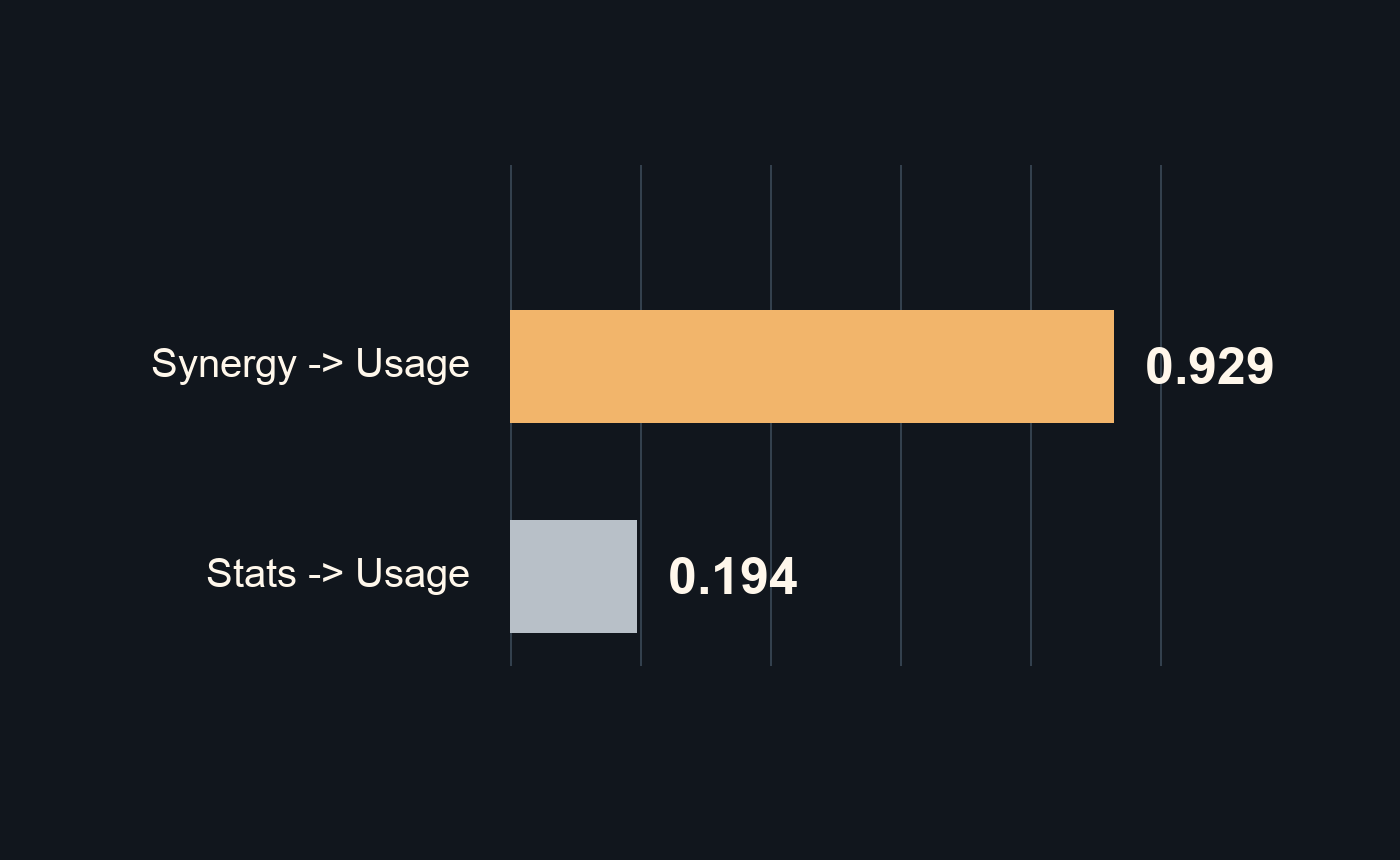
\includegraphics[width=0.58\linewidth]{correlation_insight.png}

  \small Figure 2. Preliminary correlations guide the story: total stats have a weak relationship with usage, while team connectivity is much more aligned with usage.
\end{center}
\vspace{-0.6em}

Significant changes since the proposal include a stronger focus-and-context structure, linked scatterplot-network-detail selection, an interactive Pokemon picker, network legends, an Incineroar-centered narrative reveal, build usage in the detail panel, and brushed scatterplot selections that highlight matching network nodes. We also clarified the design rule that additional charts should not overpower the network.

\section{Preliminary Results}

The current data supports the project claim. Across the cleaned usage-tracked data, total base stats and usage have a weak correlation of 0.194. Team connectivity degree and usage have a much stronger correlation of 0.903. This does not prove that connectivity alone causes success, but it strongly supports our narrative direction: competitive relevance is better explained when we include team relationships.

The case studies make this interpretable. Zacian Crowned Sword is powerful by both stats and usage, so it matches the beginner assumption. Zamazenta Crowned Shield and Mewtwo challenge the assumption because they have very high stats but low usage in this dataset. Incineroar is the main reveal: it has a moderate 530 base stat total, but high usage, many teammate connections, and a support build pattern centered on role value. Its common moves and ability provide a concrete explanation for why it fits many teams.

\section{Evaluation Plan}

We will evaluate the system through both design checks and small user feedback. First, we will perform a task-based walkthrough with classmates or teammates. We will ask whether users can answer: (1) why raw stats alone are insufficient, (2) why Incineroar is an important contradiction case, (3) what an edge means in the network, and (4) how brushing the scatterplot changes the network. Second, we will inspect whether selections remain synchronized across views and whether labels, legends, and annotations are readable on common laptop and presentation screen sizes.

Success criteria are narrative clarity rather than raw feature count. A successful viewer should leave with the idea that competitive strength is relational. If users treat the app like a broad Pokedex browser, the design has failed. If they can explain how usage, teammates, builds, and network position support the claim, the design is working.

\section{Plan of Activities}

\small
\begin{tabularx}{\linewidth}{@{}p{0.23\linewidth}p{0.18\linewidth}p{0.19\linewidth}X@{}}
\toprule
Task & Responsible & Status & Time / notes \\
\midrule
Data cleaning and validation & Team 13 & Complete & Cleaned CSV outputs and validation script are finished. \\
React + D3 prototype & Team 13 & Complete & Core scatterplot, network, picker, linked selection, brushing, and detail panel are implemented. \\
Narrative pacing and annotations & Team 13 & Ongoing & Add more controlled story states, short callouts, and transition timing without adding chart clutter. \\
Responsive polish and readability & Team 13 & Ongoing & Improve label placement, mobile layout, legends, and presentation-screen legibility. \\
Evaluation walkthrough & Team 13 & Upcoming & Run task-based feedback with classmates or teammates and record issues. \\
Final report and video/demo prep & Team 13 & Upcoming & Update final report, citations, limitations, screenshots, and speaking script. \\
\bottomrule
\end{tabularx}
\normalsize

\section{Team Effort Distribution}

All team members have contributed a similar amount of effort so far. Work has been shared across data preparation, visualization design, implementation, writing, and presentation planning. Before final submission, we will update this statement if the effort distribution changes substantially.

\section{References}
\vspace{-0.6em}
\renewcommand{\refname}{}
\bibliographystyle{plain}
\bibliography{references}

\end{document}
